\section{Hit rates}
\label{sec:hitrates}

The majority of hits in the MDTs and CSCs are due to \textit{cavern background}, not muons. Cavern background is a mixture of prompt particles from a recent proton collisions and long-lived particles accumulated from many collisions before and after the collision of interest. The most abundant particles in the cavern background are low energy photons, neutrons, and electrons, among other charged particles.

Hit rates are defined as the number of hits recorded in a given detector element divided by the livetime and active area of that detector element. The livetime is the amount of time for which the detector element is active and recording data around the proton collision of interest. The livetime of the MDTs (CSCs) is taken to be 1300 (140) ns, or 52 (5.6) bunch crossings, and the active area of each detector is derived by summing up the active area of each detector element. In the case of the MDTs, the detector elements are cylindrical tubes with a diameter of typically 3 centimeters and a length of about 1 meter. For the CSCs, these are strips with a pitch of 5 millimeters and a length of about 1 meter.

The hit rates for MDT and CSC chambers in Run 284285, which was among the longest and highest luminosity runs in 2015, are shown in Figure~\ref{fig:hitrates-vs-region-raw}. The average instantaneous luminosity in this run is $\mathcal{L}=4.1\times10^{33}$. The reported hit rate includes all $\phi$-sectors for the given $\eta$ station. The regions furthest from the interaction point, such as the MDT BOL and BOS chambers, record the smallest hit rate. The regions closest to the beampipe, such as the CSC, MDT EIL, and MDT EIS chambers, record the largest hit rate. The behavior of the hit rates is broadly consistent with previously measured rates \cite{ATL-COM-MUON-2013-003,ATL-COM-MUON-2013-011}.

\begin{figure}
  \begin{center}
    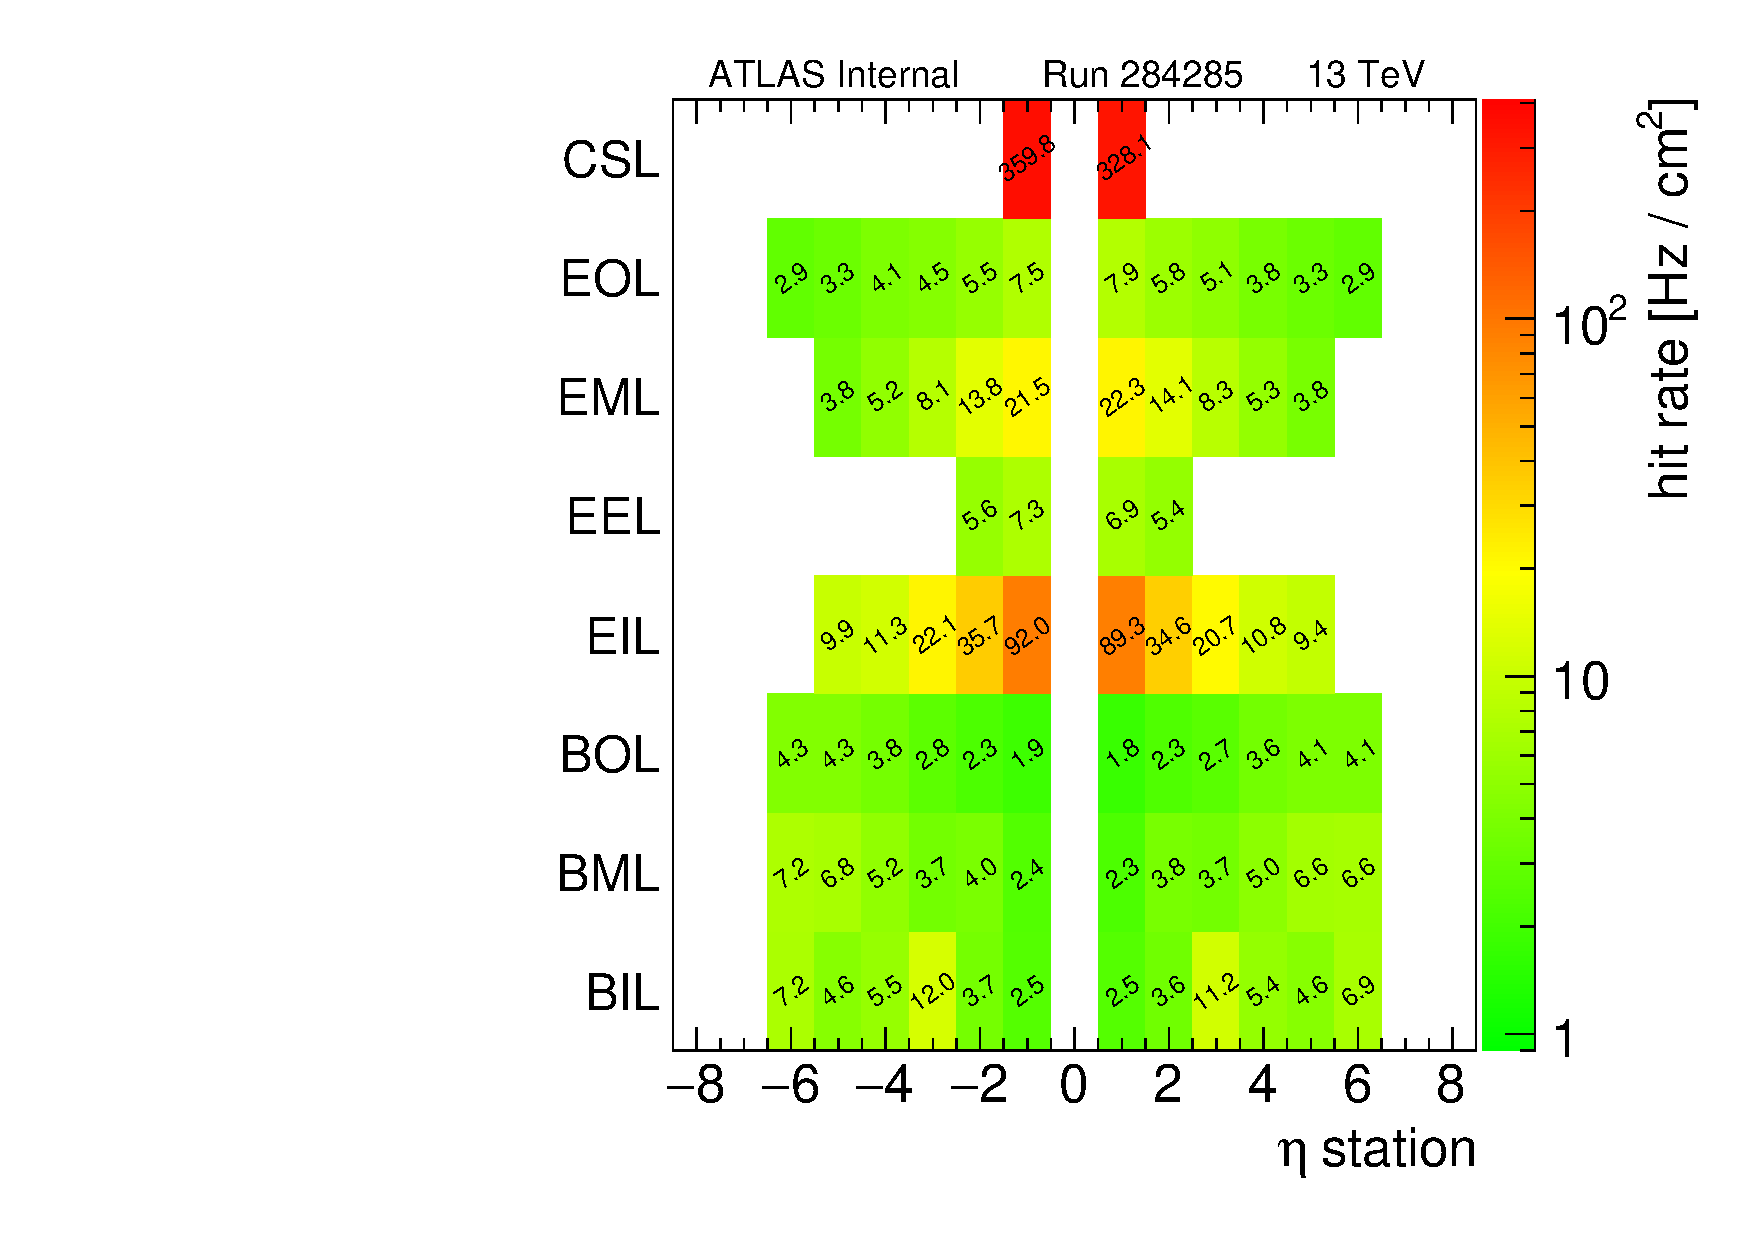
\includegraphics[width=0.45\textwidth]{./figures/rate_raw_vs_region_L_00284285.pdf}
    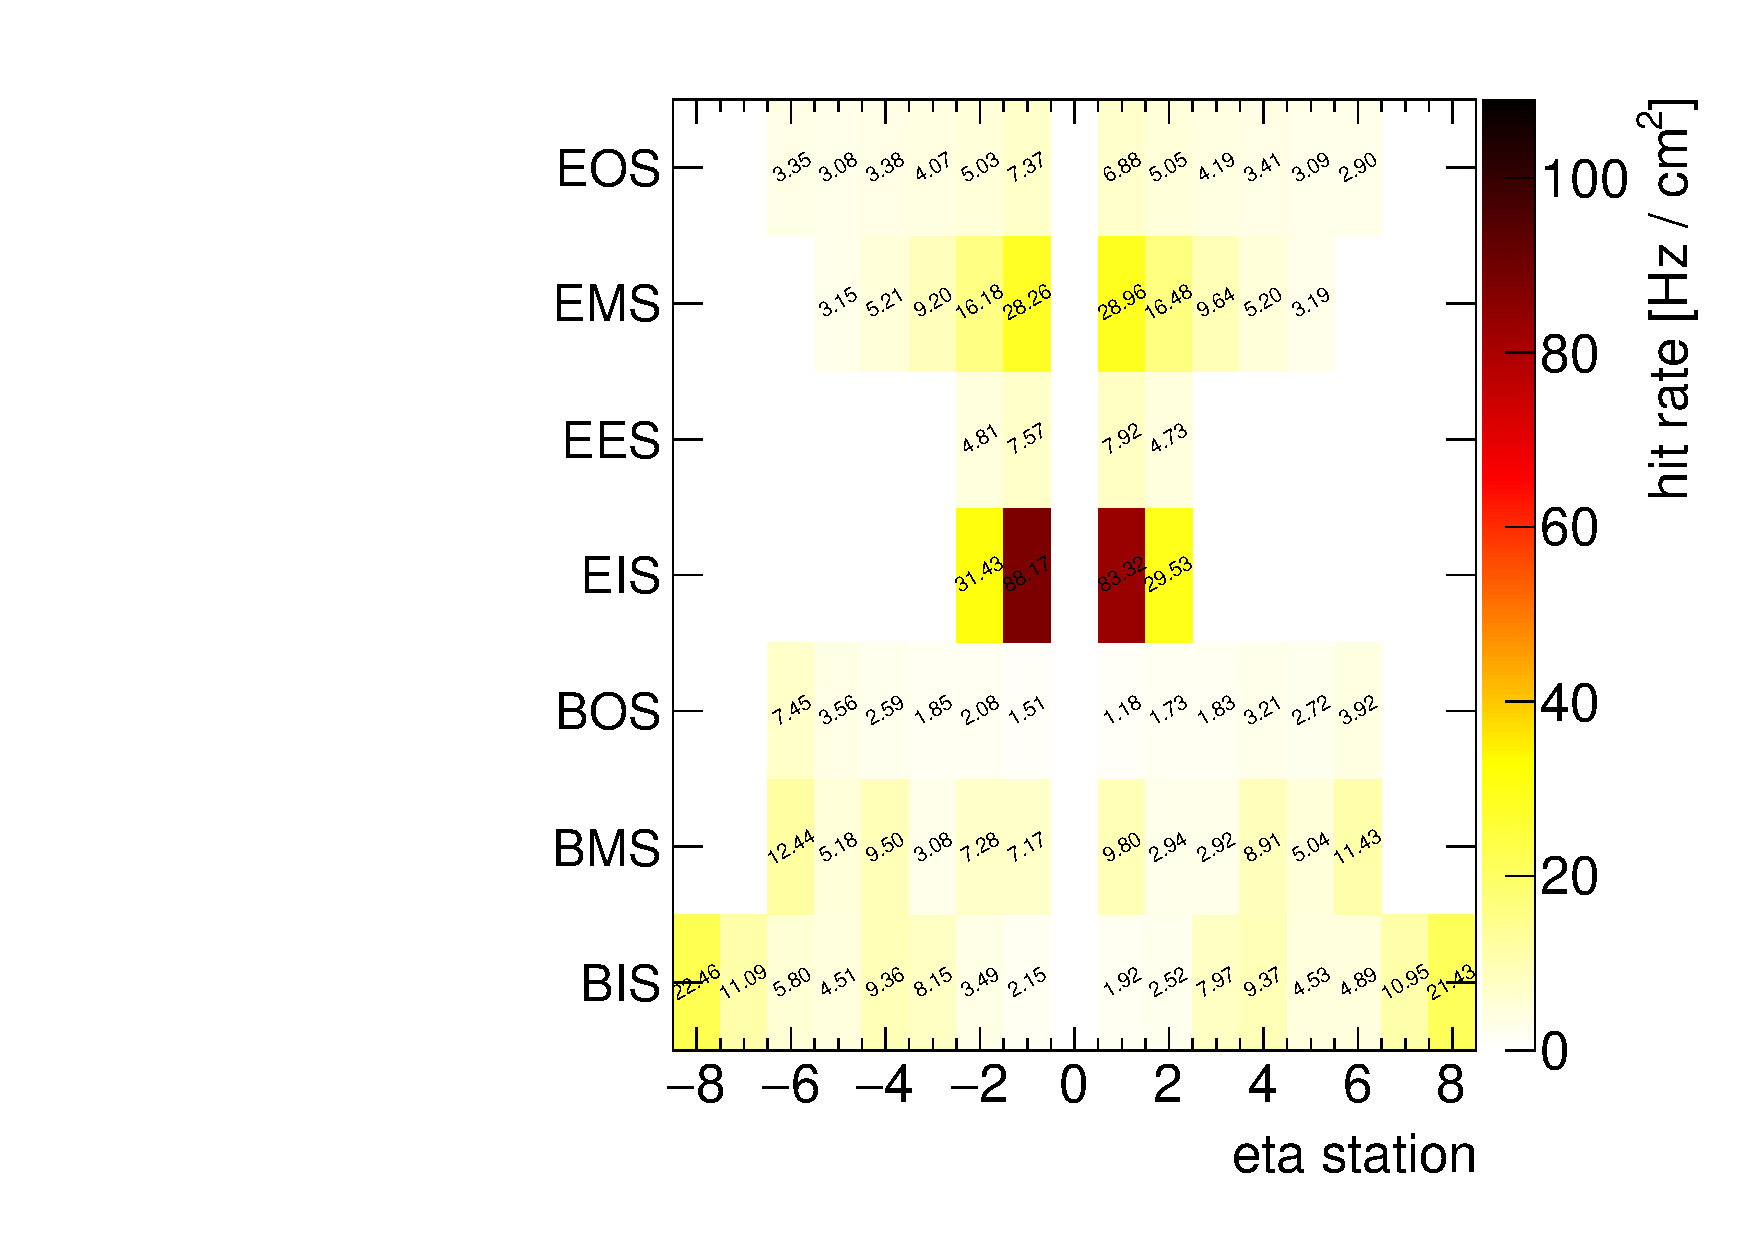
\includegraphics[width=0.45\textwidth]{./figures/rate_raw_vs_region_S_00284285.pdf}
    \caption{Total hit rate in the CSCs and MDTs in Run 284285 in the largest regions of the detector. The rates are split into large sectors (left) and small sectors (right). Positive eta stations indicate the $+z$ side of ATLAS, and negative eta stations indicate the $-z$ side.}
    \label{fig:hitrates-vs-region-raw}
  \end{center}
\end{figure}

The regions of the MDTs and CSCs with the highest rate are of special interest because the harsher conditions probe the data-taking capacity of the detectors. The hit rate as a function of instantaneous luminosity in this regions is measured to gauge the detector performance in the presence of increasing particle flux, since the instantaneous luminosity is linearly proportional to the number of interactions in a proton bunch crossing.

The hit rates for the CSC L and S chambers, MDT EIL1 and EIS1 chambers, and MDT EML1 and EMS1 chambers are shown as a function of the instantaneous luminosity in Figures~\ref{fig:hitrates-vs-lumi-csc-raw}, \ref{fig:hitrates-vs-lumi-mdt-ei1-raw}, and \ref{fig:hitrates-vs-lumi-mdt-em1-raw}, respectively. Linear fits are overlaid and provide a reasonable description of the data. The hit rates show strong dependence on the number of filled bunches in the LHC. The hit rates do not show non-linear behavior, such as saturation, at the highest instantaneous luminosity reached in 2015. This indicates robust MDT and CSC operation during 2015 data-taking.

\begin{figure}
  \begin{center}
    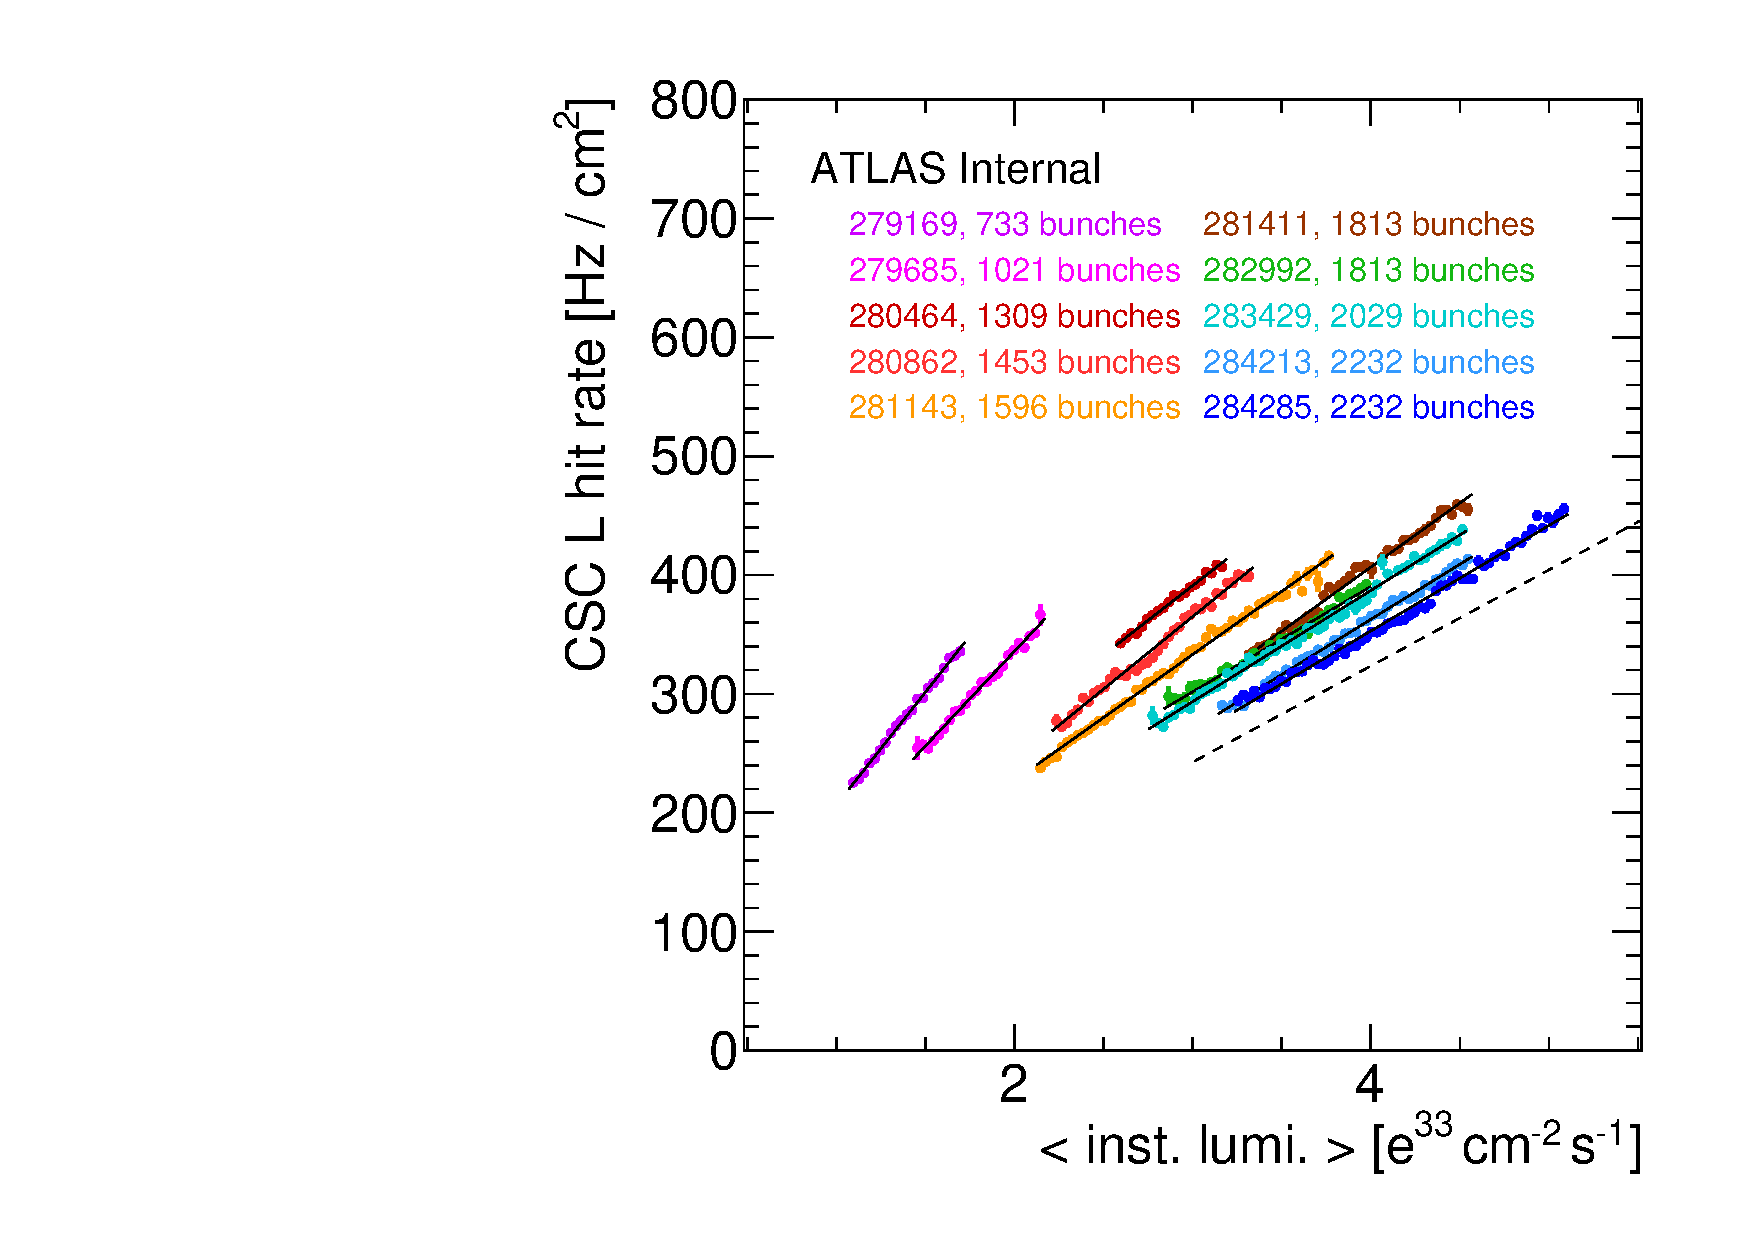
\includegraphics[width=0.45\textwidth]{./figures/rate_raw_vs_lumi_vs_evts_csc_CSL1_overlay.pdf}
    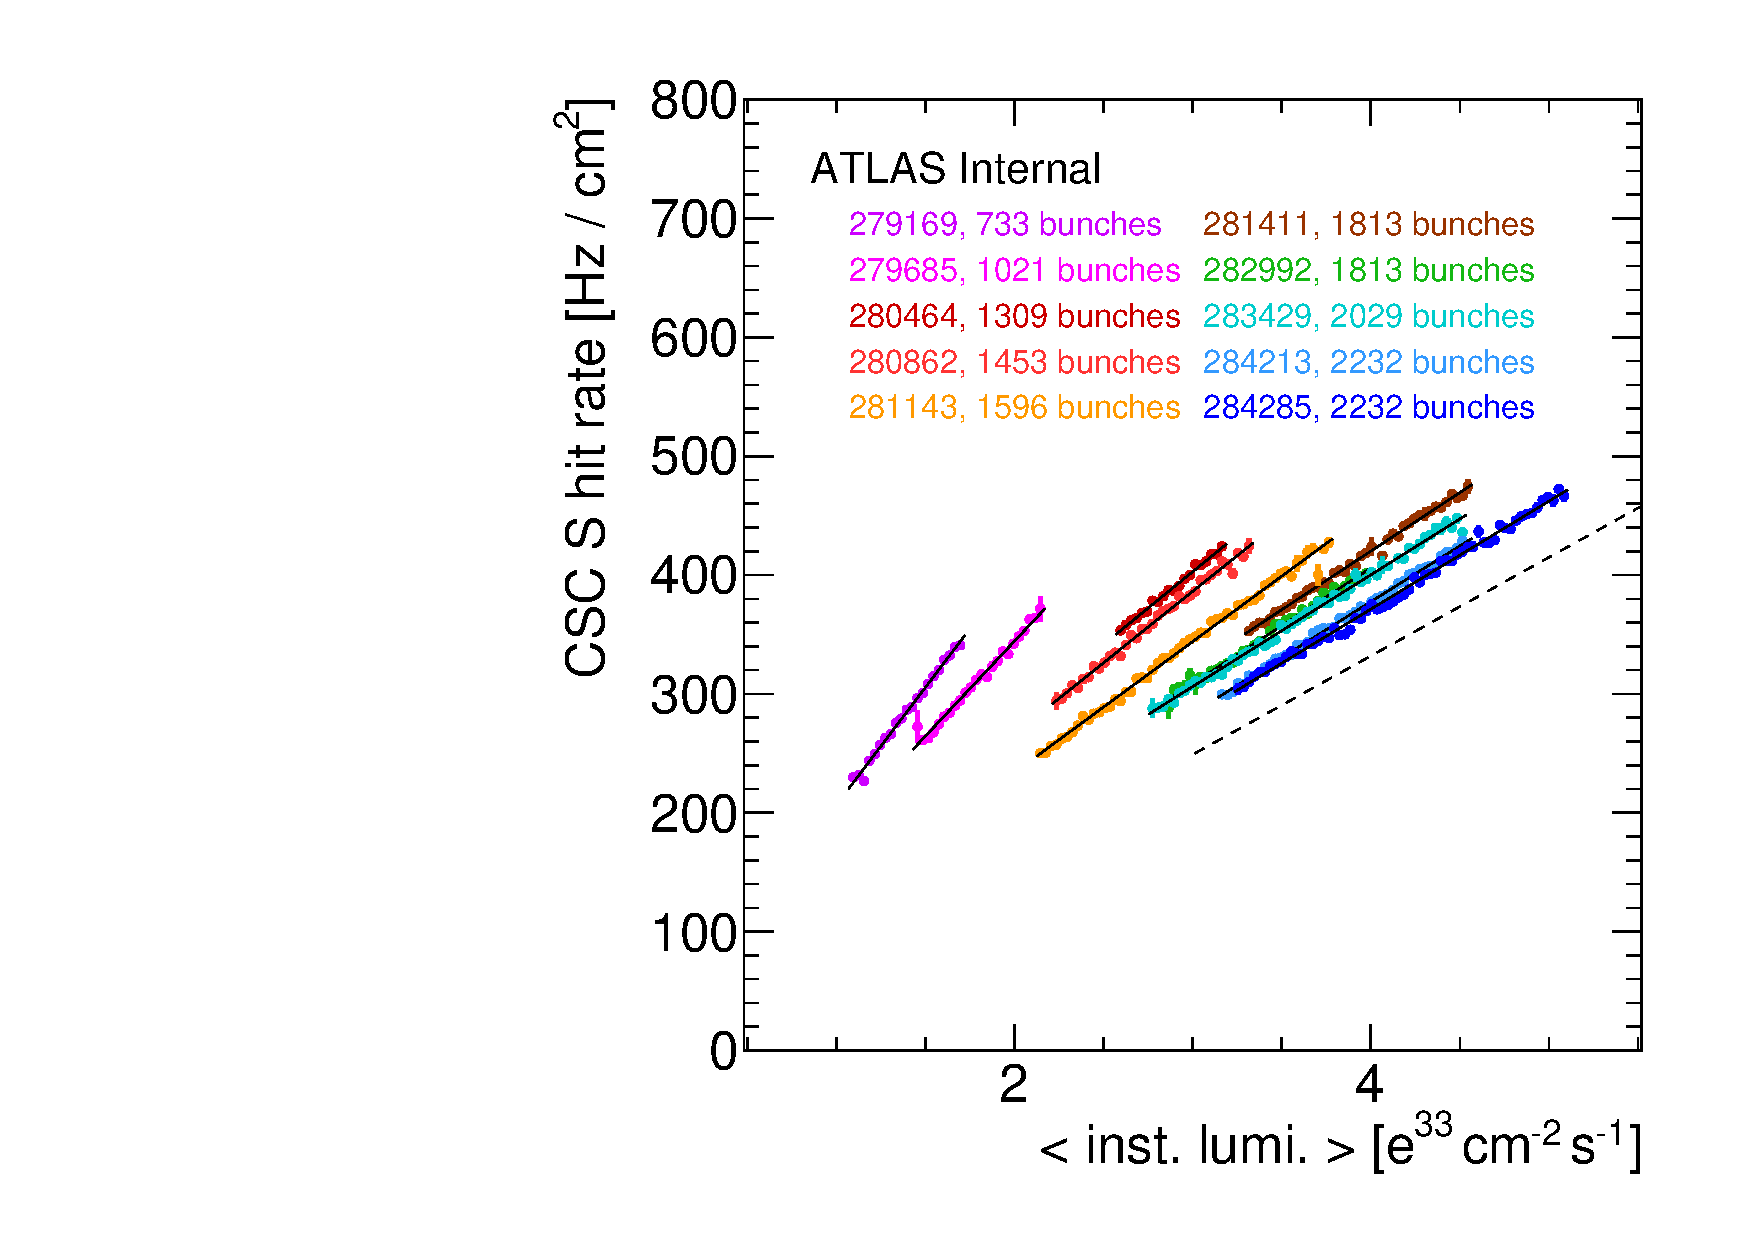
\includegraphics[width=0.45\textwidth]{./figures/rate_raw_vs_lumi_vs_evts_csc_CSS1_overlay.pdf}
    \caption{Total hit rate in the CSC large (left) and small (right) chambers as a function of instantaneous luminosity, for multiple runs.}
    \label{fig:hitrates-vs-lumi-csc-raw}
  \end{center}
\end{figure}

\begin{figure}
  \begin{center}
    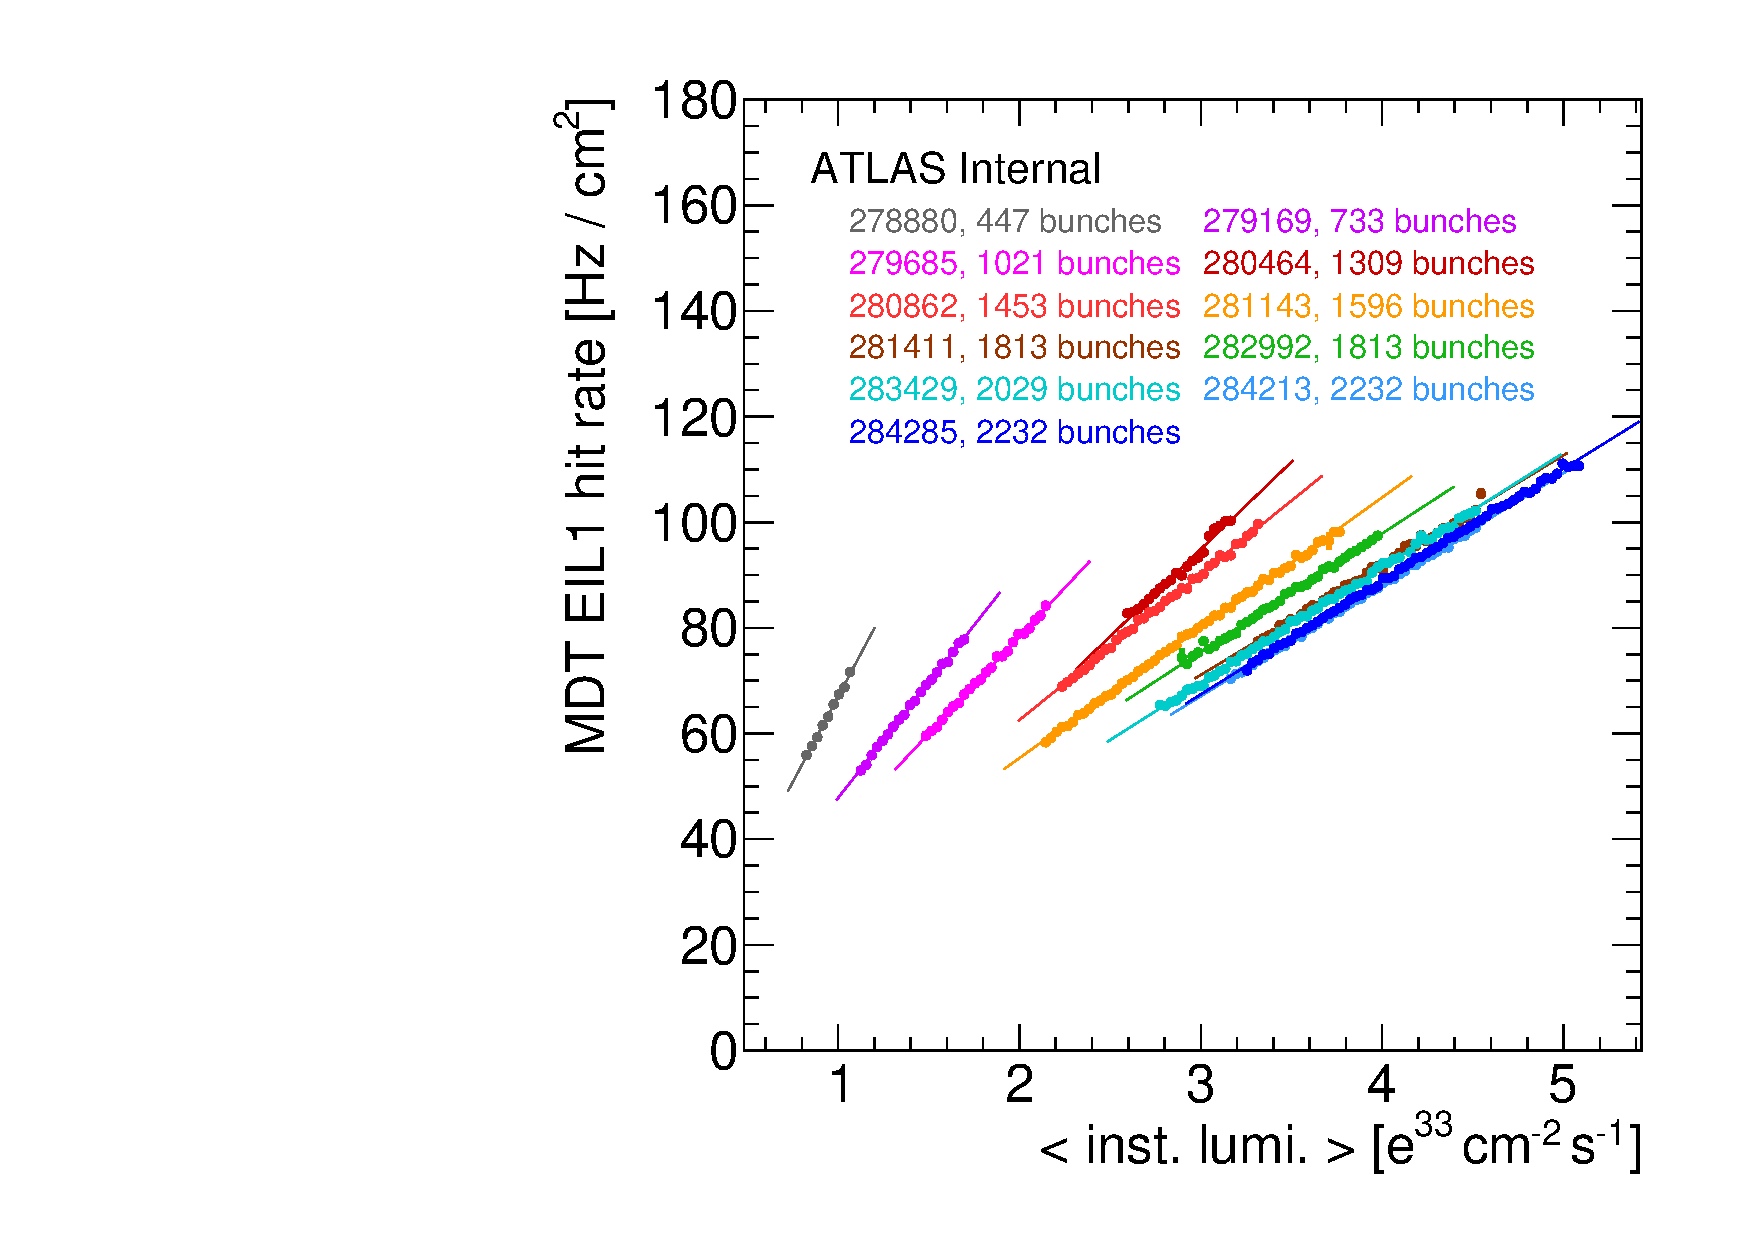
\includegraphics[width=0.45\textwidth]{./figures/rate_raw_vs_lumi_vs_evts_mdt_EIL1_overlay.pdf}
    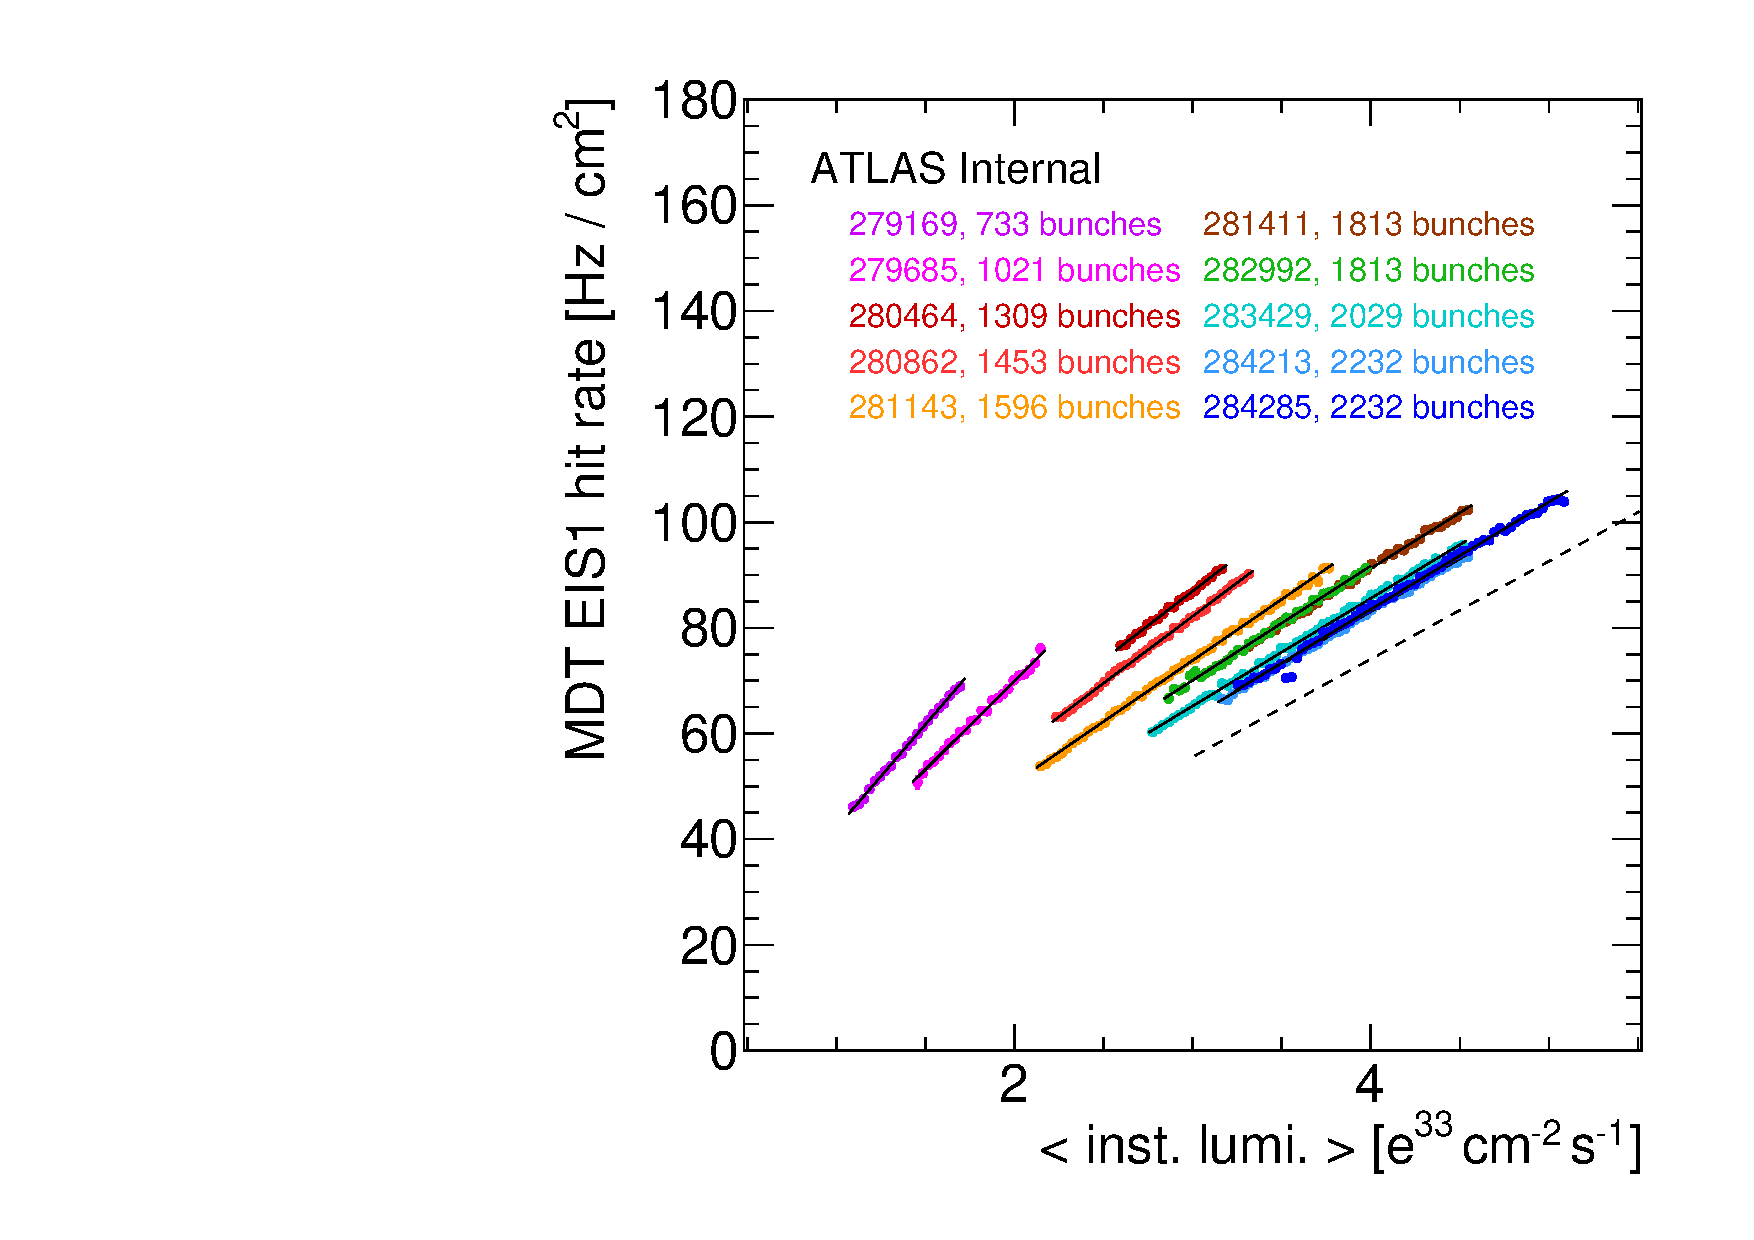
\includegraphics[width=0.45\textwidth]{./figures/rate_raw_vs_lumi_vs_evts_mdt_EIS1_overlay.pdf}
    \caption{Total hit rate in the MDT EI large (left) and small (right) chambers as a function of instantaneous luminosity, for multiple runs.}
    \label{fig:hitrates-vs-lumi-mdt-ei1-raw}
  \end{center}
\end{figure}

\begin{figure}
  \begin{center}
    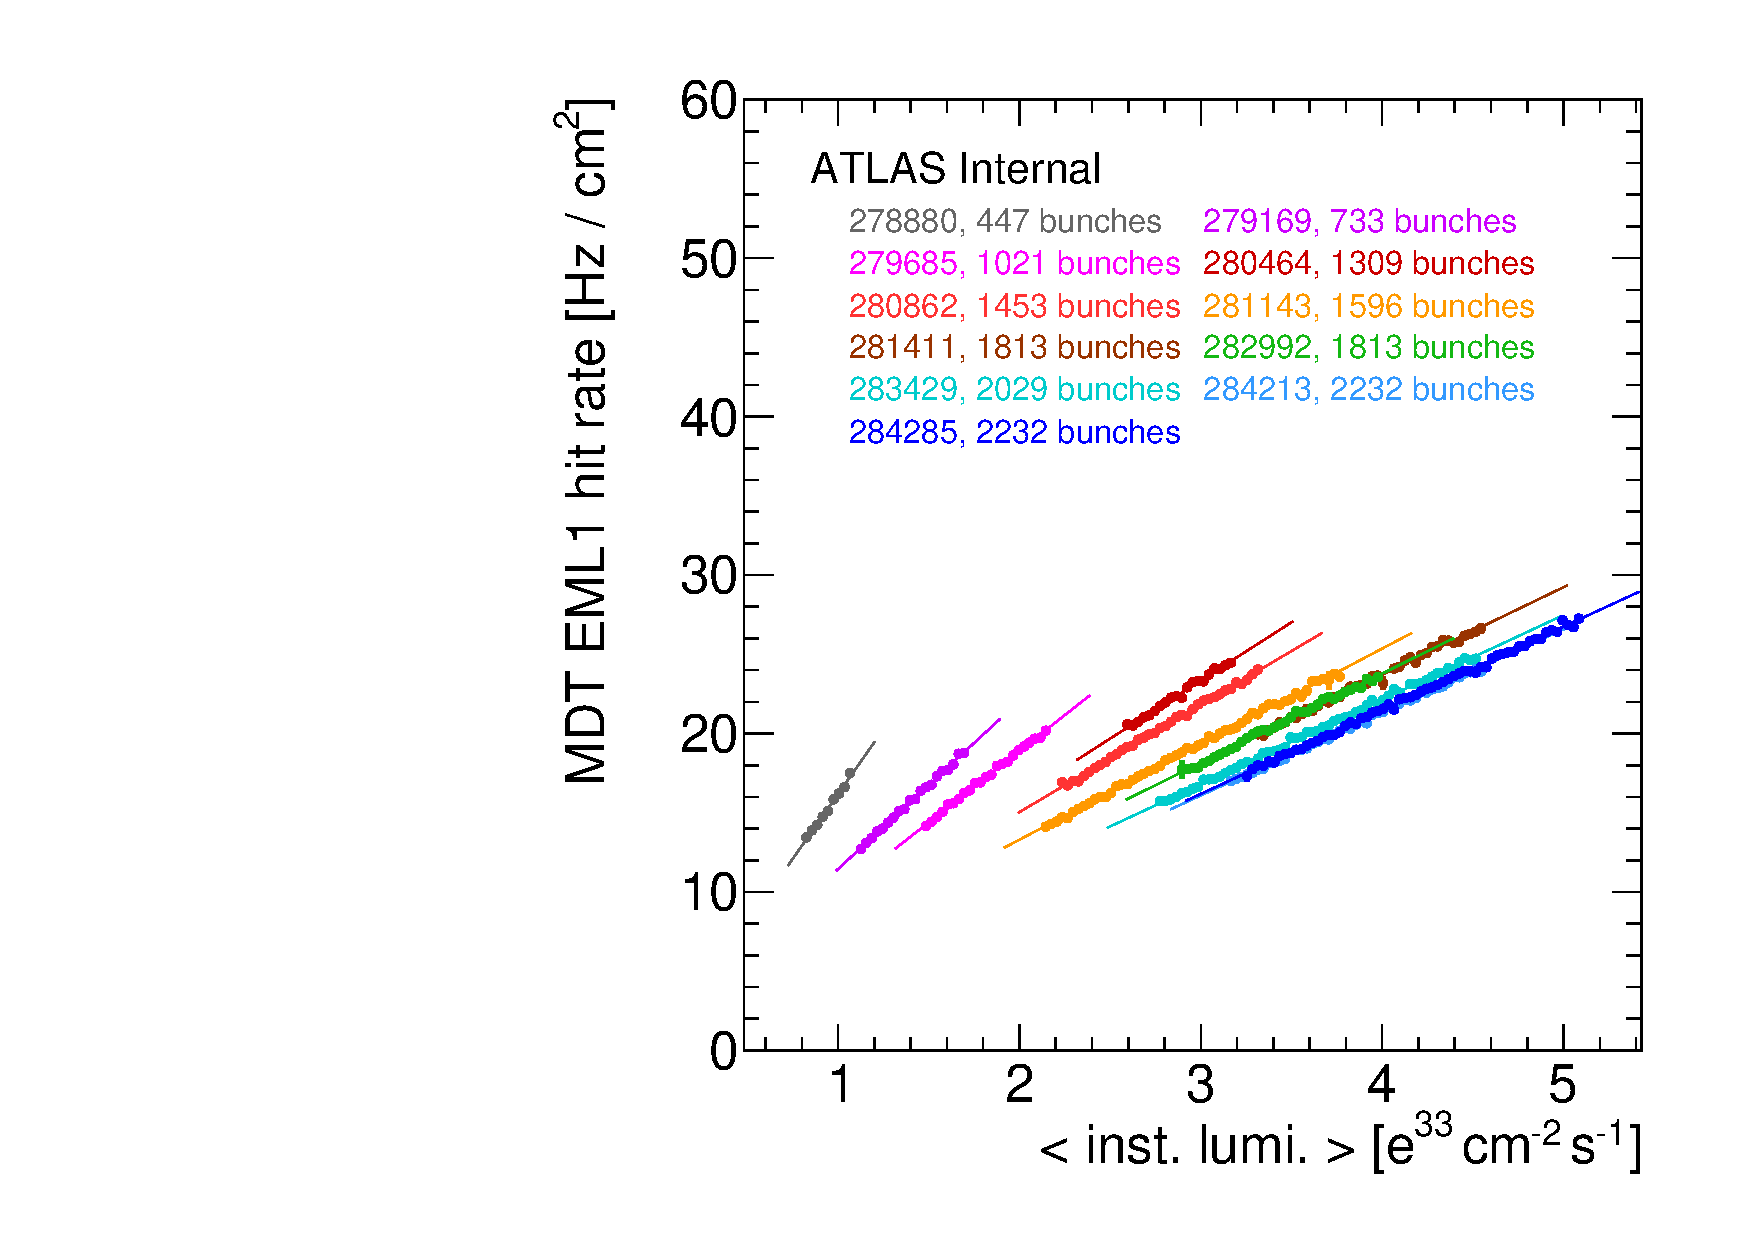
\includegraphics[width=0.45\textwidth]{./figures/rate_raw_vs_lumi_vs_evts_mdt_EML1_overlay.pdf}
    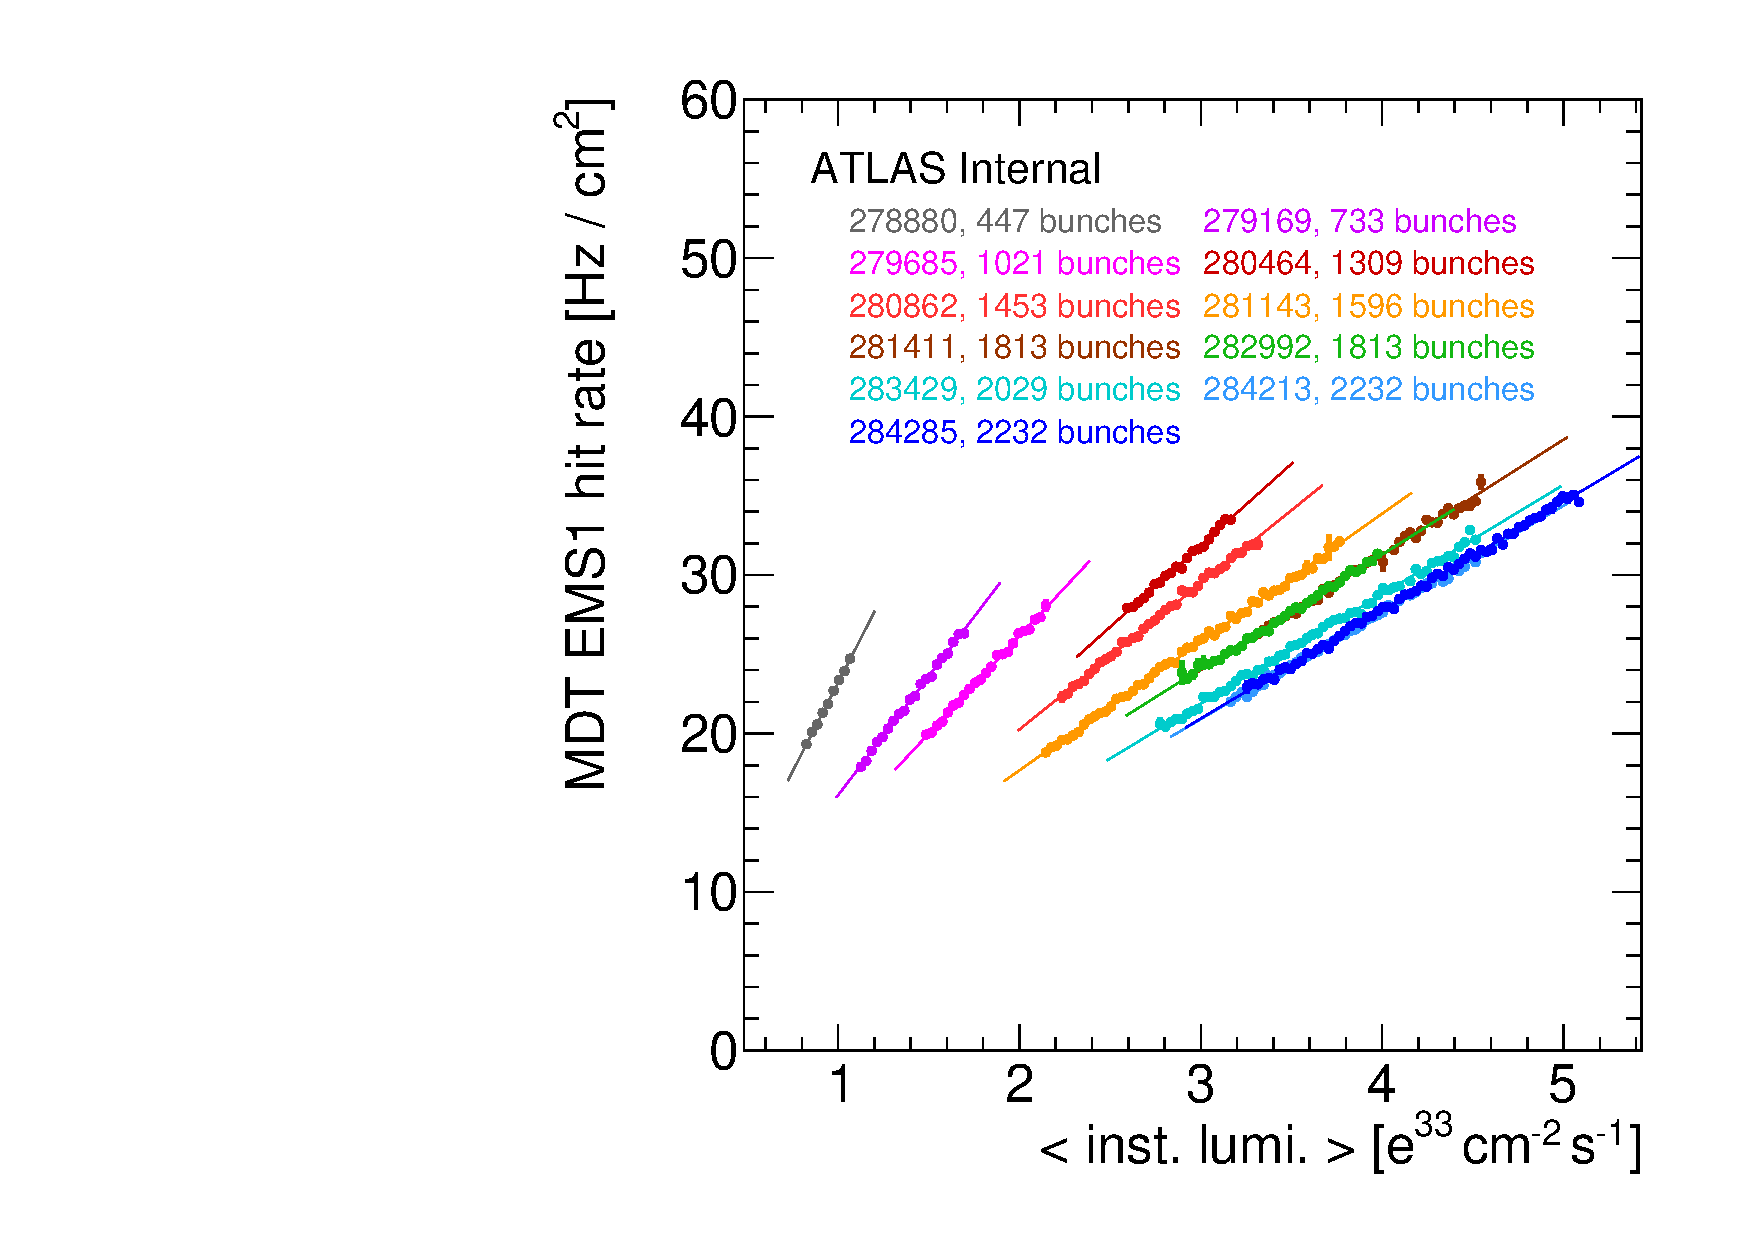
\includegraphics[width=0.45\textwidth]{./figures/rate_raw_vs_lumi_vs_evts_mdt_EMS1_overlay.pdf}
    \caption{Total hit rate in the MDT EM large (left) and small (right) chambers as a function of instantaneous luminosity, for multiple runs.}
    \label{fig:hitrates-vs-lumi-mdt-em1-raw}
  \end{center}
\end{figure}

In the endcap chambers, the hit rate depends significantly on the transverse distance $r$ from the beampipe. This is shown in Figure~\ref{fig:hitrates-vs-r-raw} for Run 284285 in the inner endcap, which includes CSC, MDT EIL1 and EIS1, and MDT EIL2 and EIS2 chambers. The CSC hit rates are as large as 800 $\text{Hz} / \text{cm}^2$ closest to the beampipe and as small as 150 $\text{Hz} / \text{cm}^2$ furthest from the beampipe. Exponential fits as a function of $r$ are overlaid and provide a reasonable description of the data. A comparison of the average and peak hit rates in the CSCs are sumarized in Table~\ref{tab:hitrates-vs-r-raw}.

\begin{figure}
  \begin{center}
    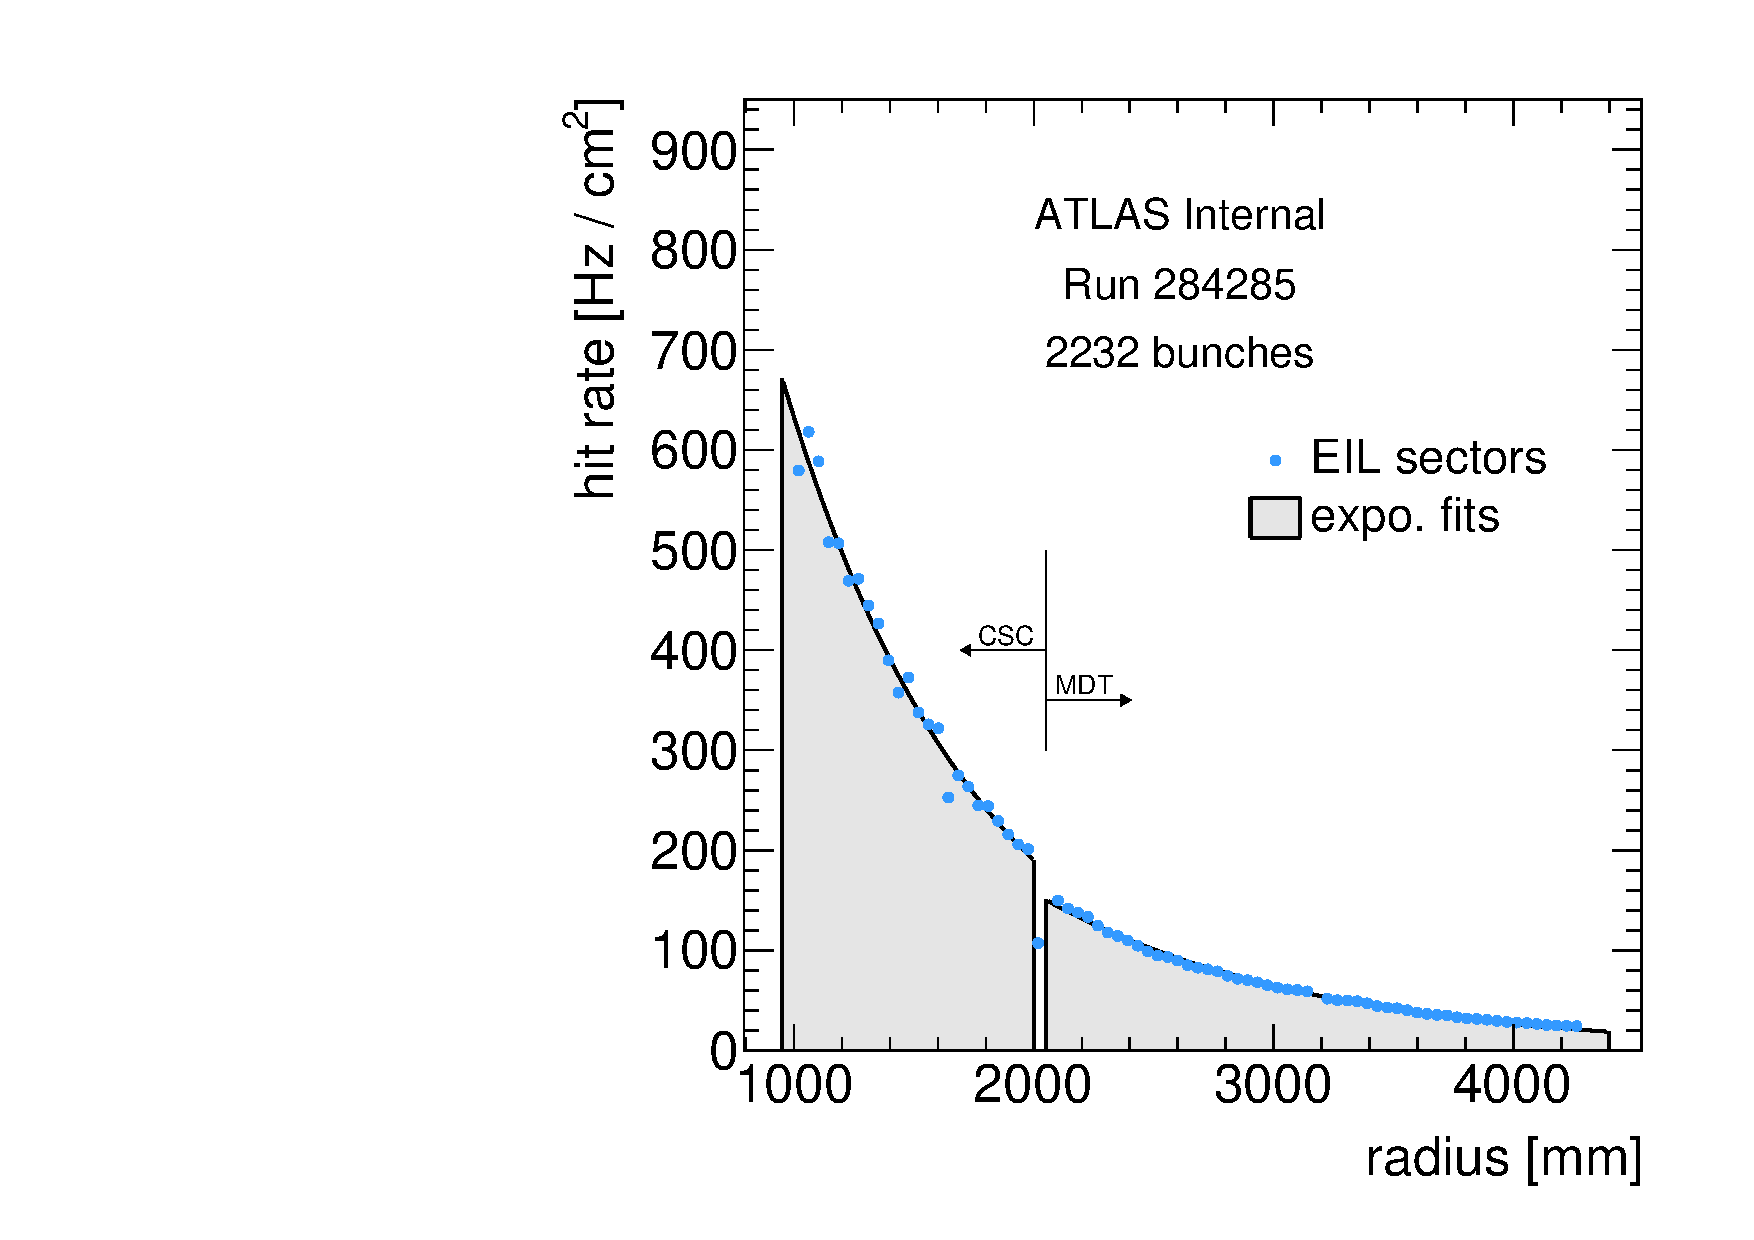
\includegraphics[width=0.45\textwidth]{./figures/rate_raw_vs_r_EIL_00284285.pdf}
    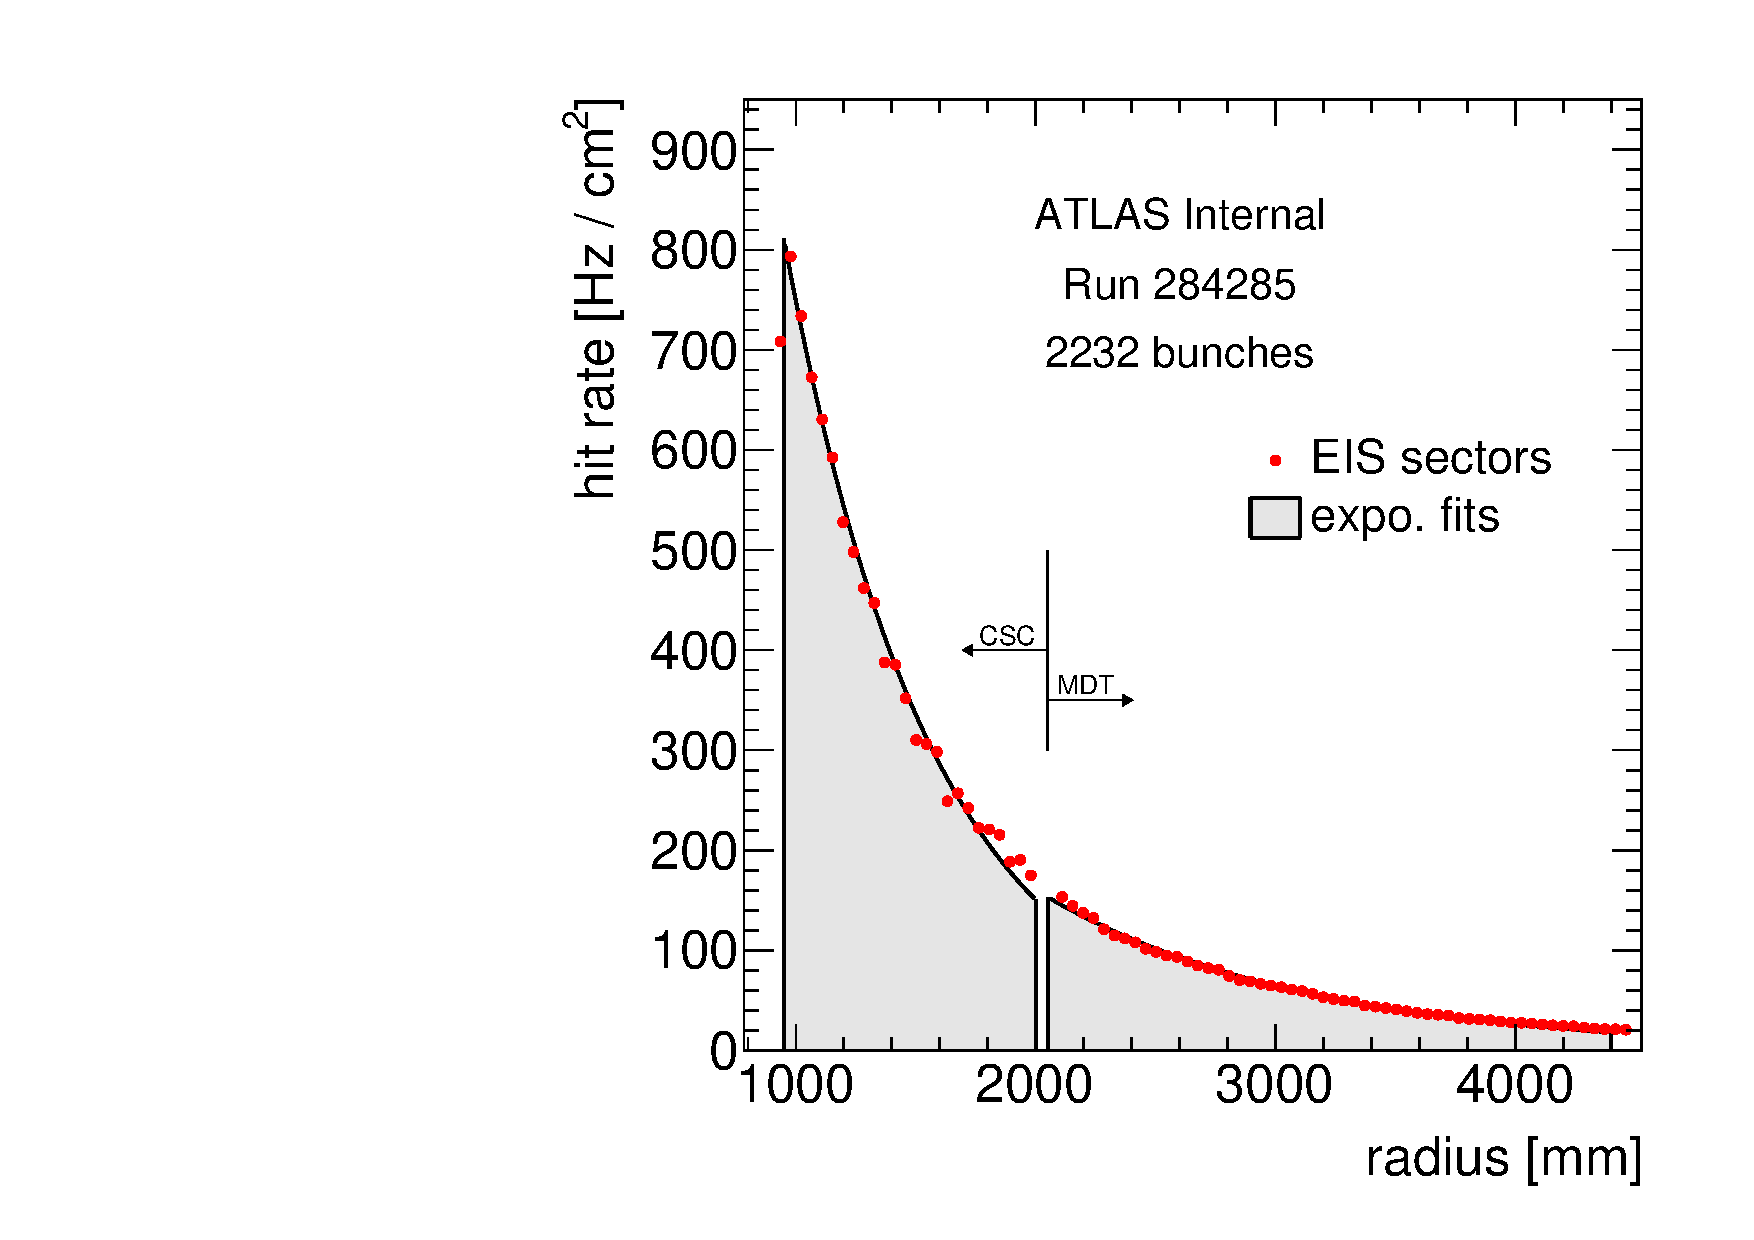
\includegraphics[width=0.45\textwidth]{./figures/rate_raw_vs_r_EIS_00284285.pdf}
    \caption{Total hit rate as a function of the transverse distance from the beam pipe in the small wheel, for large (left) and small (right) sectors, in Run 284285.}
    \label{fig:hitrates-vs-r-raw}
  \end{center}
\end{figure}

\newcommand*{\hspsix}{\hspace*{0.6cm}}

\begin{table}
  \begin{center}
    \renewcommand{\arraystretch}{1.4}
    \begin{tabular}{c|c|c|c|c}
      \multicolumn{2}{c|}{}                                             & \multicolumn{2}{c|}{\rate}                   & \multicolumn{1}{c}{} \\
      \hspsix region \hspsix & expo. fit                                & \hspsix average \hspsix & peak: smallest $r$ & peak / average \\
      \hline\hline
      CSC L                  & $e^{\ 7.65\ -\ 1.20\cdot r \text{ [m]}}$ & 344                     & 668                & 1.94 \\
      CSC S                  & $e^{\ 8.22\ -\ 1.61\cdot r \text{ [m]}}$ & 360                     & 803                & 2.23 \\
    \end{tabular}
    \caption{Comparison of the CSC chamber average hit rate with the hit rate closest to the beampipe in Run 284285. The average luminosity in Run 284285 is $\mathcal{L}=4.1\times10^{33}$.}
    \label{tab:hitrates-vs-r-raw}
  \end{center}
\end{table}

